\section{Theory}

\begin{frame}{Quantum State Tomography}
  \begin{itemize}
  \item \textbf{Fundamental Problem:} Measurement doesn't reveal the quantum state
  \item \textbf{Solution:} Repeated measurement in different bases $\rightarrow$
      reconstructed state
  \end{itemize}
  \vspace{0.5cm}

  \begin{columns}
    \column{0.5\textwidth}
    \centering \textbf{1-qubit reconstruction}
      \begin{equation*}
        \rho=\frac{1}{2}\left(\mathbb{1}+\sum_{i=1}^3\alpha_i\sigma_i\right)
      \end{equation*}
      \begin{equation*}
        \rho=\frac{1}{2}\left(\mathbb{1}
          + \langle \hat{X} \rangle \hat{X}
          + \langle \hat{Y} \rangle \hat{Y}
          + \langle \hat{Z} \rangle \hat{Z} \right)
      \end{equation*}

      \vspace{0.7cm}
      Total of 3 different sets of measurements.

    \column{0.5\textwidth}
    \centering \textbf{2-qubit reconstruction}
    \begin{equation*}
      \rho=\frac{1}{4}\sum_{\vec{v}_i}\left\langle\sigma_{v_1}
        \otimes\sigma_{v_2}\right\rangle\sigma_{v_1}\otimes\sigma_{v_2} 
    \end{equation*}
    \begin{equation*}
      \rho=\frac{1}{4}\left(\mathbb{1} \otimes \mathbb{1}
        + \langle \mathbb{1} \otimes \hat{X} \rangle \mathbb{1} \otimes \hat{X} +
         ...\right)
    \end{equation*}

    \vspace{0.7cm}
    Total of 9 measurement set, for 15 non-trivial expectation values.

  \end{columns} 
\end{frame}


\begin{frame}{Calibrating for Readout - Single Qubit}
  \begin{itemize}
    \item The act of measurement on superconducting qubits introduces a large
source of error.
    \item We correct for this by initializing and measuring empty circuits.
  \end{itemize}

\begin{columns}
  \column{0.5\textwidth}
  \begin{block}{Scheme to Calibrate}
    \begin{itemize}
    \item Initialize in $\ket{0}$, $\ket{1}$.
    \item Measure output and derive $\epsilon$ values.
    \end{itemize}
  \end{block}

  \column{0.5\textwidth}
  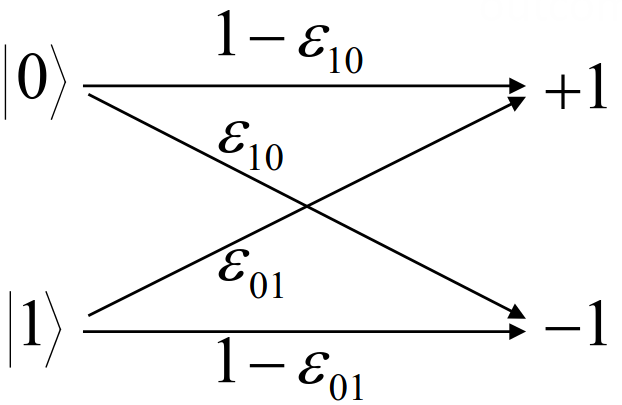
\includegraphics[width=\textwidth]{images/bit_flip_calibration.png}
\end{columns}

\begin{equation*}
  \overline{m}=\left(\epsilon_{01}-\epsilon_{10}\right)
  +\left(1-\epsilon_{01}-\epsilon_{10}\right)\left(\left|\alpha\right|^2
    -\left|\beta\right|^2\right)
\end{equation*}
\begin{equation}
  \begin{split}
    \left\langle \hat{\sigma}_i\right\rangle=
    \frac{\overline{m}_i-\beta_0}{\beta_1}
  \end{split}
\end{equation}
\end{frame}

\begin{frame}{Calibrating for Readout - 2 Qubit Case}
  Much less straightforward...
  
  \begin{equation*}
    \label{beta}
    \begin{split}
      \begin{pmatrix}
        \overline{m}_{ij,MSQ} \\ \overline{m}_{ij,LSQ} \\ \overline{m}_{ij,corr}
      \end{pmatrix} =
      \begin{pmatrix}
        \beta_{0,M} \\ \beta_{0,L} \\ \beta_{0,corr}
      \end{pmatrix} + 
      \begin{pmatrix}
        \beta_{1,M}&\beta_{2,M}&\beta_{3,M} \\
        \beta_{1,L}&\beta_{2,L}&\beta_{3,L} \\
        \beta_{1,corr}&\beta_{2,corr}&\beta_{3,corr}
      \end{pmatrix}
      \begin{pmatrix}
        \left\langle I\sigma_j\right\rangle \\ \left\langle
          \sigma_iI\right\rangle \\ \left\langle \sigma_i\sigma_j\right\rangle
      \end{pmatrix}
    \end{split}
  \end{equation*}

In order to find the corrected expectation values from the measured ones (the
$\bar{m}$), we need to find the $\beta$ values by initializing the qubits in
$\ket{00}$, $\ket{01}$, $\ket{10}$, and $\ket{11}$ and relating the output
expectation values using:
  
\begin{equation}
  \begin{pmatrix}
    \overline{m}_{A,k} \\ \overline{m}_{B,k} \\ \overline{m}_{C,k}
    \\ \overline{m}_{D,k}
  \end{pmatrix} =
  \begin{pmatrix}
    1&1&1&1\\
    1&1&-1&-1\\
    1&-1&1&-1\\
    1&-1&-1&1
  \end{pmatrix}
  \begin{pmatrix}
    \beta_{0,k} \\ \beta_{1,k} \\ \beta_{2,k} \\ \beta_{3,k}
  \end{pmatrix}
\end{equation}
where the $k$ can be MSQ, LSQ or the correlated outcomes.

\end{frame}
  
\section{Superconducting Qubits}

\begin{frame}{Quantum LC oscillators}
\begin{columns}
  \column{0.5\textwidth}
  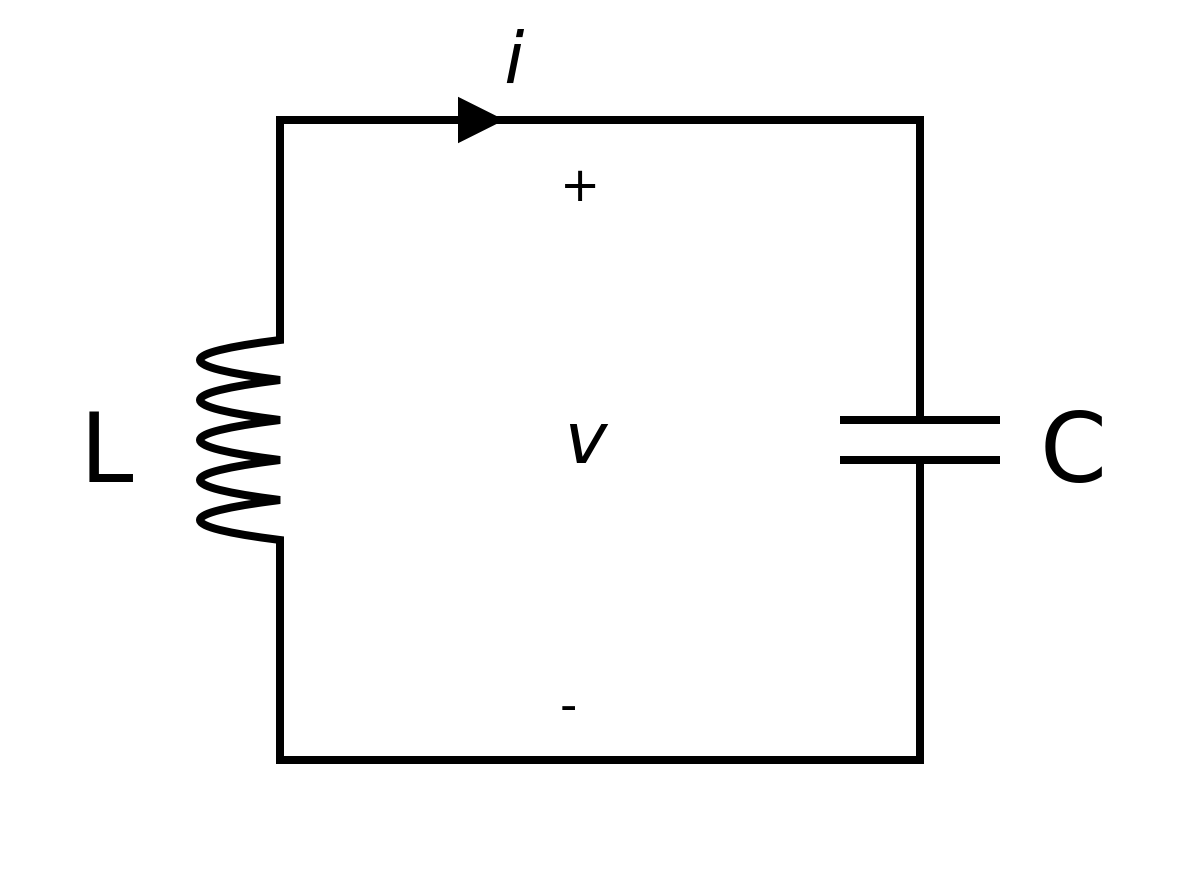
\includegraphics[width=\textwidth]{images/lc_circuit.png}

  Physics described by the HO Hamiltonian:
  \begin{equation*}
    \begin{aligned}
    H &= \frac{1}{2} C V^2 + \frac{1}{2} L I^2 \\
      &= \frac{Q^2}{2C} + \frac{\phi^2}{2L}
    \end{aligned}
  \end{equation*}

  \column{0.5\textwidth}
  \textbf{Energy Levels}
  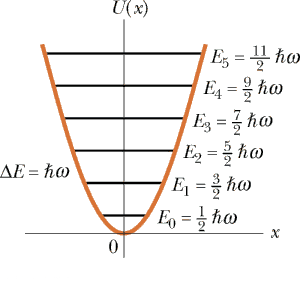
\includegraphics[width=\textwidth]{images/harm_osc_energies.png}

  Energy spacing is \textbf{even}... not good for a qubit!
\end{columns}

\end{frame}

\begin{frame}{The Transmon Qubit}
  \begin{itemize}
  \item \textbf{First Step:} Introduce Josephson element with non-linear
inductance to shift energy levels.
  \item \textbf{Make it a Transmon:} Couple to regular LC circuit to reduce
    sensitivity to charge noise, by boosting the ratio $\nicefrac{E_J}{E_C}$.
    Increases $T_1$ coherence times.
  \end{itemize}

  \begin{columns}
    \column{0.5\textwidth}
    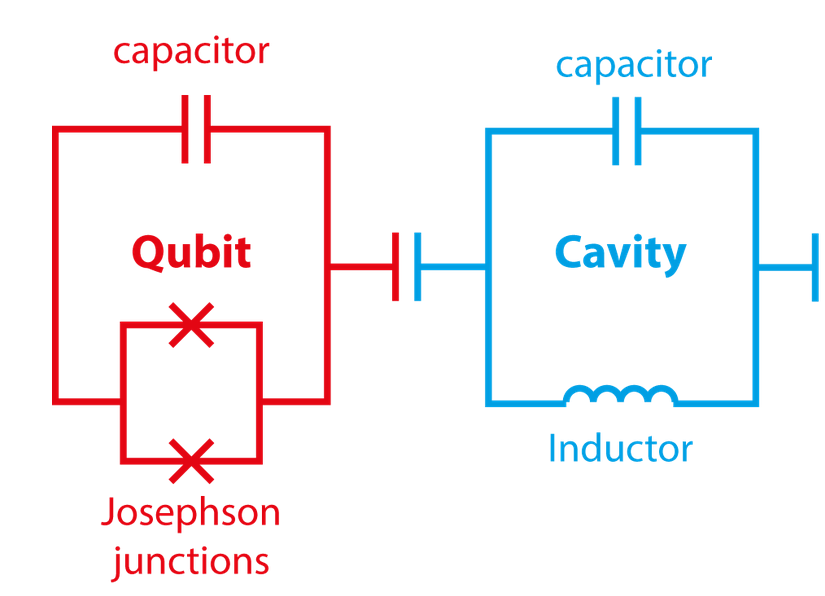
\includegraphics[width=\textwidth]{images/transmon_diagram.png}

    Unique energy spacing $\rightarrow$ confine dynamics to 2 states, $\ket{0}$
    and $\ket{1}$

    \column{0.5\textwidth}
    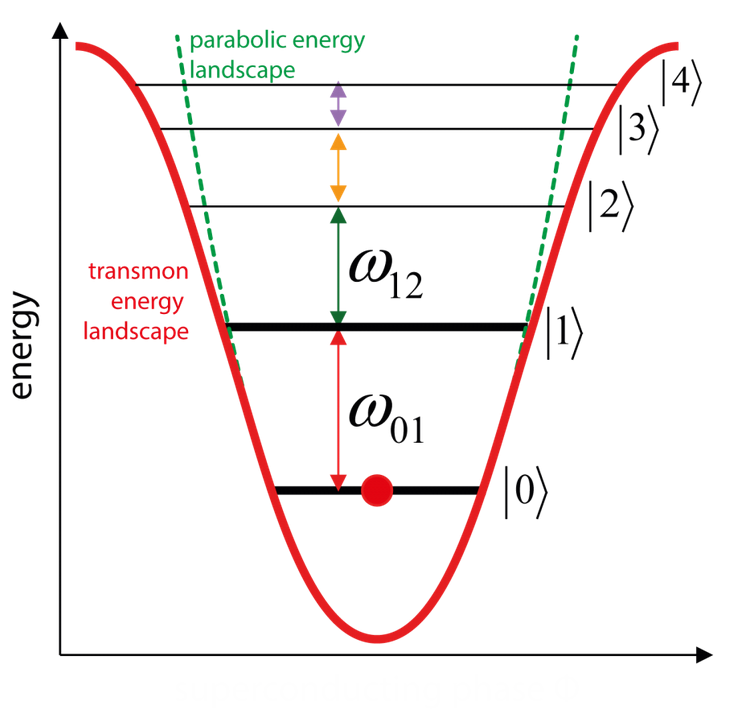
\includegraphics[width=\textwidth]{images/energy_spacing_transmon.png}

  \end{columns}
\end{frame}
  

%%% Local Variables:
%%% mode: latex
%%% TeX-master: "presentation"
%%% End:
